\documentclass[review]{siamart}

% 1. Preamble and packages
\usepackage{lipsum}
\usepackage{amsfonts}
\usepackage{graphicx}
\usepackage{algorithmic}
\usepackage{amsopn}
\usepackage{booktabs}

\newcommand{\bes}{\begin{equation*}}
\newcommand{\ben}[1]{\begin{equation}\label{#1}}
\newcommand{\ees}{\end{equation*}}
\newcommand{\be}{\begin{equation}}
\newcommand{\ee}{\end{equation}}

% 2. Paper title
\newcommand{\TheTitle}{%
The Multilevel Summation Method: An Introductory Look and Python Experiments (Draft 2)
}

% 3. Your Name
\newcommand{\TheName}{%
  Josh Bevan
}

% 4. Your Email
\newcommand{\TheAddress}{\email{%
    jjbevan2@illinois.edu
}}

% ---------------------------------------------
% ---------------------------------------------
\author{\TheName\thanks{\TheAddress}}
\title{{\TheTitle}}
\headers{\TheTitle}{\TheName}
\ifpdf%
\hypersetup{%
  pdftitle={\TheTitle},
  pdfauthor={\TheName}
}
\fi

\begin{document}

\maketitle

\vspace{1cm}
% ---------------------------------------------
% ---------------------------------------------

% [20 of 100] Problem Statement
%   - What is the problem/method/application that you are studying?
%   - Why is this important or interesting?
%   - What are a few related concepts?  (This does not need to be an exhaustive literature survey -- but some context is necessary)
%   - What are the details of the problem/method/application (enough to make a convincing case that you know what you're doing)
% [20 of 100] Approach
%   - How will you study this problem?
%   - If it's a method you're studying, what are you testing and why?
%   - If it's an application that you're studying, what method(s) will you use and why?
% [30 of 100] Numerical Results
%   - Show some numerical results.
%   - Discussion the numerical results.
%   - Show that you understand the numerical results.
%   - Did make sensible numerical tests?
% [10 of 100] Concluding remarks
%   - Critique the methods that you employed.
%   - What worked well?
%   - What did not?
%   - What would you like to do with more time?
% [10 of 100] General readability and presentation
%   - Did you use clean, easy-to-read figures?
%   - Was your write-up easy-to-follow?
%   - Was your write-up less than or equal to 8 pages (including figures/references)?
%   - Did you make a convincing case?
% [10 of 100] Code
%   - Did you include code and did your code execute what you claim?
%
% [100 of 100] Total

%--------------------------------------------
\section{Problem Statement}\label{sec:problem}
There are many physical phenomena that fit into the category of $n$-body problems, systems where there are long-range pairwise interactions between each body. These include areas like molecular dynamics, electro-magnetics, gravitation, and fluid flow. The simulation of these phenomena can be computationally intensive if all pairwise interactions are calculated directly. Direct calculation requires calculations that scale as $\mathcal{O}(n^2)$. For many such simulations of practical consequence $n$ can be on the order of millions, rendering direct approaches useless.

Fast methods seek to reduce the computational cost to  $\mathcal{O}(n log n)$ or even  $\mathcal{O}(n)$ by replacing direct evaluation of long-range interactions with approximations. The two sets of method choices can be roughly lumped into two categories: periodic and non-periodic. Periodic approaches include techniques like Particle Mesh Ewald (PME) which can employ periodic basis functions, but place periodicity requirements on the solution domain. The other set of methods include tree codes and most famously the Fast Multipole Method (FMM). In contrast to PME etc. the FMM is applicable for non-periodic domains.

In contrast to these examples the Multilevel Summation Method (MSM) has several advantages. Multipole methods don't have explicit continuity of the potential  in the transition from the near-field to the regions well separated from the target. In comparison to PME, MSM benefits from exact calculation of short-range interactions as well as naturally separating the potential into different length skills which more readily permits multiple time stepping.\cite{2}

The following section presents the MSM in greater detail, though it is by no mean comprehensive. The intent is to highlight the salient features of the MSM and then present some experiments in Python that implement/illustrate the concepts.

%--------------------------------------------
\section{Approach}\label{sec:main}
In many cases the potential to be calculated can be expressed as:
\be E(x) = C \sum_{i=1}^N \sum_{j=1}^N q_i q_j k(r_i,r_j)\ee
where $q$ represents the strength of some property (e.g. charge, mass) and $r$ is the position vector for a given particle.

The function $k(r_i, r_j)$ is the interaction kernel, in many cases the Green's function that describes the fundamental behavior of solutions to the governing equation. For electrostatics and gravitation it is simply $1/r$. Issues arise if the kernel is simply used without accounting for the difficulty in approximating the near singular parts. Approximations for long-range interactions depend upon the availability of good approximations. Therefore a splitting is necessary to be able to separately manipulate only the smooth components.

We can rewrite the kernel as a sum of kernels of increasing reach and reducing variation. Take for example a particular splitting case\cite{3} with four terms:
\be \frac{1}{z} = f_0(z)+f_1(z)+f_2(z)+f_3(z) \ee
where we have made the substitution $z = |r-r'|$ and we assume the kernel functions under consideration is radial, that is $k(r,r') \rightarrow f(|r-r'|)=f(z)$.

The shortest range part is $f_0$ on the individual particle level, and is directly calculated. The other three parts are approximated by an interpolation on a hierarchy of increasingly coarser grid. This means pairwise interactions are not dramatically reduced to only short-range interactions. A splitting parameter $a$ is used to control the spatial reach of each of the coarser kernels. In this example then the other terms would have ranges $a$, $2a$, and $4a$.

This leaves the issue of actually constructing each of these kernels. Consider an unknown smoothing function $g_a(r,r')$, with the property:
\be g_a(r,r') = \frac{1}{z} \;\; \text{for} \;\; z>a \ee
while for z<a there is less variation compared ot the original potential.

If this smoothing function is used one receives a telescoping sum that satisfies the original equation:
\be f_0(z) = 1/z - g_a(r,r') \ee
\be f_1(z) = g_a(r,r')-g_{2a}(r,r') \ee
\be f_2(z) = g_{2a}(r,r')-g_{4a}(r,r') \ee
\be f_3(z) = g_{4a}(r,r') \ee

Unsurprisingly the smoothness of the kernel is dependent on the smoothing function. Ideally a given $g_a$ should be selected to be within the range of interpolation on the grid. It is worth noting that so far no approximations have been made, merely decomposed the original kernel into a more suggestive form. The actual approximations are made during the interpolation of the smooth kernels to the hierarchal grids; typically with a nodal basis defined on the grid. As an example the first interpolation of the first smooth kernel would have the form:
\be g_a(r,r') \approx \sum_n \sum_m \phi_n(r) g_a(r_n,r_m) \phi_m(r') \ee
where $r_n / r_m$ are grid points and $\phi_n/\phi_m$ are the nodal basis functions.

We can now substitute this approximation expression into our pairwise interaction problem to yield:
\be C \sum_{i=1}^N \sum_{j=1}^N q_i q_j g_a(r_i,r_j) \approx C \sum_{i=1}^N \sum_{j=1}^N q_i q_j\sum_n \sum_m \phi_n(r) g_a(r_n,r_m) \phi_m(r') \ee
however our nodal basis functions are compactly supported on just the grid, so the two sets of sums reduce to:
\be  = C \sum_{n}^N \sum_{m}^N q_n^h q_m^h g_a(r_n,r_m) \ee
where we now have approximate grid charge values that are the interpolation of the underlying particles:
\be q_n^h = \sum_{i=1}^N q_i \phi_n(r_i) \ee

The result is the reduction from pairwise particle interactions to pairwise grid interactions. One interesting feature of this is that even if the particles may move, the interpolated grid locations used in the decomposition don't.

For coarser levels, $g_{2a}$ for example, interpolation is again performed but with larger mesh spacing (double in the case of $g_{2a}$)
\be C \sum_{i=1}^N \sum_{j=1}^N q_i q_j g_{2a}(r_i,r_j)  = C \sum_{i=1}^N \sum_{j=1}^N q_n^{2h} q_m^{2h} g_{2a}(r_{2n},r_{2m}) \ee

We now have all the parts necessary to compute the potential field $E$. For the finest level, compute:
\be e_{short} =K(x)q \ee
where K is matrix constructed from the shortest range kernel $f_0$ and q are the particles that directly participate in the short-range interactions. Moving up the hierarchy:
\be q^h = (I_h)^T q \;\; e^h_{short} = K_hq^h \ee
\be q^{2h} = (I_{2h}^h)^T q \;\; e^{2h}_{short} = K_{2h}q^{2h} \ee
\be q^{4h} = (I_{4h}^{2h})^T q \;\; e^{4h}_{short} = K_{4h}q^{4h} \ee
and then back down
\be e^{4h} = e^{4h}_{short} \ee
\be e^{2h} = e^{2h}_{short} + I^{2h}_{4h}e^{4h} \ee
\be e^{h} = e^{h}_{short}+I^h_{2h}e^{2h} \ee

We now have all components needed to calculate E:
\be \frac{1}{2}q\, e_{short} + q \, I_h \, e^h \ee

Figure 1 diagrammatically shows the cycle following these steps. For the particle and grid levels and the calculation of each level's component contribution.

\begin{figure}[!htb]
\centering
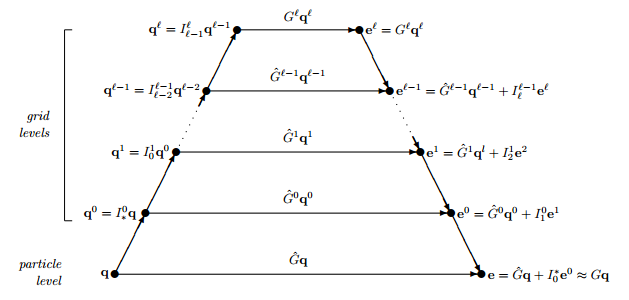
\includegraphics[width=0.8\textwidth]{levels.PNG}
\caption{Hierarchal decomposition of potential into two parts: close range interaction and smooth long-range interactions which can be approximated by an interpolation.\cite{3}}
\end{figure}

%--------------------------------------------
\section{Numerical Results}\label{sec:num}
The smoothing operation has been implemented for the solver to be used in the splitting. An example comparison of the pre/post-smoothing is shown in Figure 2. The routines to generate interpolation operators are mostly done as well. Time permitting additional smoothing routines will be added so that several can be compared to determine their comparative impacts.

The kernel matrix generation routines still need to be completed and the main driver script that cycles up and back down the MSM needs to have either a recursive setup, or for simplicity a fixed number of levels hard coded. Any numerical investigations will have a gentle number of points, so the hierarchy won't need to be particularly deep.



\begin{figure}[!htb]
\centering
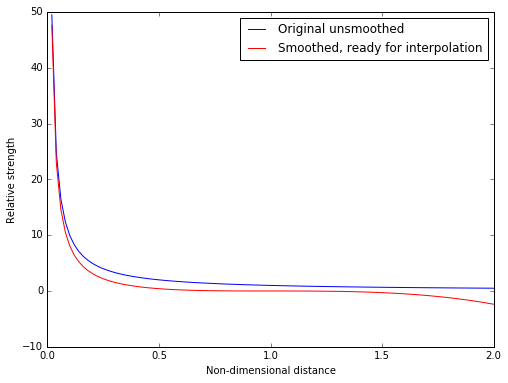
\includegraphics[width=0.6\textwidth]{smooth.PNG}
\caption{Comparison of original and smoothed interaction for a single particle.}
\end{figure}

%--------------------------------------------
\section{Conclusions}\label{sec:conc}
The multilevel summation method provides an alternate means of efficiently evaluating n-body problems. Also, in comparison to a FMM there are fewer components necessary for an efficient implementation. The underlying algorithm and most of the implementation details are now understood for this project and the remaining parts of the solver will be finished. A suitable set of tests will be performed to evaluate performance, contingent upon the currently unknown efficiency/robustness of this implementation.

%--------------------------------------------
\begin{thebibliography}{3}
\bibitem{1}
 David J. Hardy, Zhe Wu, James C. Phillips, John E. Stone, Robert D. Skeel, and Klaus Schulten. Multilevel Summation Method for Electrostatic Force Evaluation. Journal of Chemical Theory and Computation 2015 11 (2), 766-779 DOI: 10.1021/ct5009075
\bibitem{2}
Hardy, D. J. Multilevel summation for the fast evaluation of forces for the simulation of biomolecules. Ph.D. thesis, University of Illinois at Urbana−Champaign, Champaign, IL, 2006; Also Department of Computer Science Report No. UIUCDCS-R-2006-2546, May 2006.
\bibitem{3}
Bond, Stephen D. Multilevel summation methods for efficient evaluation of long-range pairwise interactions in atomistic and coarse-grained molecular simulation. No. SAND2014-0355. Sandia National Laboratories (SNL-NM), Albuquerque, NM (United States), 2014.
\bibitem{4}
Skeel, Robert D., Ismail Tezcan, and David J. Hardy. "Multiple grid methods for classical molecular dynamics." Journal of Computational Chemistry 23, no. 6 (2002): 673-684.

\end{thebibliography}

\end{document}
